\chapter{Resultados}

%El dispositivo fabricado tiene las caracter\'isticas detalladas en la tabla \ref{tabla:caracteristicas_fabricado}. 

%\begin{table}
%		\begin{center}
%			\caption{Caracter\'isticas del dispositivo fabricado.}
%			\label{tabla:caracteristicas_fabricado}
%			\small
%			\begin{tabular}{r|m{7cm}}
%				\toprule
%				\textbf{Caracter\'istica} & \textbf{Descripci\'on}\\
%				\midrule
%				Unidad de procesamiento & 	System On Chip formado por un microcontrolador Atmel ATMega128 y un radio transceptor ZigBee 802.15.4 a 2.4 GHz\\
%				Perif\'ericos & 5 puertos digitales I/O, 18 puertos multifunci\'on (PWM, ADC, INT), 1 puerto RS-232, 1 puerto JTAG y 1 puerto SPI\\
%				\bottomrule			
%			\end{tabular}
%		\end{center}
%\end{table}

\section{Verificaci\'on de funcionamiento del dispositivo}

El proceso de validaci\'on consiste en una serie de pruebas a los distintos componentes que lo forman, las cuales se listan a continuaci\'on:

\begin{itemize}
\item Verificaci\'on f\'isica del dispositivo y comprobaci\'on de funcionamiento en el rango de voltaje esperado, 
\item Verificaci\'on del funcionamiento del microcontrolador, 
\item Medici\'on de consumo de corriente, 
\item Medici\'on de alcance de radio comunicaci\'on.
\end{itemize}

A continuaci\'on se detalla cada una de estas pruebas realizadas. 

\subsection{Verificaci\'on f\'isica del dispositivo}

Luego de la fabricaci\'on del dispositivo se realiz\'o una verificaci\'on de cortos circuitos, la prueba consiste en medir la resistencia entre la l\'inea de alimentaci\'on de voltaje y la l\'inea de tierra, esto con la finalidad de evitar da\~nos en el dispositivo al aplicar voltaje por primera vez. Tambi\'en se verificaron cortos circuitos entre las l\'ineas de comunicaci\'on serial y puertos de prop\'osito general. En estas pruebas no se encontraron errores en el dispositivo. 

% De hecho si se encontraron errores aqui, los leds estaban en la posicion incorrecta, el dispositivo se 
% envio a la fabrica para reparar el error. No es un error interesante y por lo tanto lo estoy dejando fuera de los resultados. 

Se verific\'o el voltaje de operaci\'on y se logr\'o encender el dispositivo en el rango de 3.3 a 16 Vcd.

%Para comprobar el funcionamiento del dispositivo luego de su fabricaci\'on, se le realizaron las siguientes pruebas:  

%\begin{itemize}
%\item Pruebas de funcionamiento el\'ectrico,
%\item Pruebas de funcionamiento de componentes.
%\end{itemize}

%Las pruebas de funcionamiento el\'ectrico consisten en la verificaci\'on de la operaci\'on del dispositivo en el rango de voltaje definido en la etapa de dise\~no y en la revisi\'on del consumo de corriente del dispositivo en sus distintas etapas de operaci\'on (en modo de ahorro de energ\'ia, en modo de espera y en modo de transmisi\'on de datos). 

%Por otro lado, las pruebas de funcionamiento de componentes consisten en la verificaci\'on del funcionamiento de cada uno de los componentes que forman al dispositivo. Pruebas tales como la verificaci\'on de la interfaz de programaci\'on del microcontrolador, la verificaci\'on del funcionamiento de los puertos de prop\'osito general, puerto serial y radio comunicaci\'on. 

\subsection{Verificaci\'on del funcionamiento del microcontrolador}

Una vez que se ha comprobado el funcionamiento el\'ectrico del dispositivo se verifica el estado del microcontrolador, en particular se comprueba que: 

\begin{itemize}
\item El funcionamiento de las interfaces JTAG y SPI es el adecuado. Es posible leer el identificador del microcontrolador a trav\'es de estas interfaces utilizando un programador de microcontroladores,
\item Los puertos de prop\'osito general operan correctamente presentando transiciones de 0V a VCC Vcd para estados l\'ogicos de 0 a 1 respectivamente,
\item Que el transceptor serial funciona adecuadamente haciendo posible el env\'io y recepci\'on de datos desde y hacia el dispositivo, 
\item Que el transceptor de radio frecuencia es capaz de establecer conexi\'on con otros dispositivos.
\end{itemize}

Para simplificar el proceso de pruebas, todas estas verificaciones se hicieron ejecutando la aplicaci\'on de demostraci\'on WSNDemo (ver anexo) en el dispositivo SerialDongle.

\subsection{Medici\'on de consumo de corriente}

Posteriormente se realizaron pruebas de consumo de corriente en distintas etapas de operaci\'on las cuales se clasificaron en tres tipos: 

\begin{itemize}
\item Modo de transmisi\'on de datos: Todos los componentes del dispositivo est\'an encendidos y se realiza comunicaci\'on inal\'ambrica con otro dispositivo,
\item Modo de espera: Todos los componentes del dispositivo est\'an encendidos pero no se realiza comunicaci\'on inal\'ambrica, 
\item Modo de ahorro de energ\'ia: El microcontrolador es enviado a modo de ahorro de energ\'ia, sin embargo algunos componentes externos siguen en funcionamiento. 
\end{itemize}

Utilizando la aplicaci\'on de prueba WSNDemo de BitCloud en dos dispositivos SerialDongle, se realiz\'o el siguiente experimento,

\begin{enumerate}
\item Programar un dispositivo como nodo coordinador,
\item Programar un segundo dispositivo como nodo final,
\item Encender ambos dispositivos y verificar la conexi\'on inal\'ambrica,
\item Aplicando un voltaje de 5 Vcd, se mide el consumo de corriente en ambos dispositivos. 
\end{enumerate}

Se midi\'o el consumo de corriente cuando : 

\begin{itemize}
\item El nodo coordinador est\'a en funcionamiento sin ning\'un nodo final conectado, ver figura \ref{fig:coordinador_sinnodo},
\item El nodo coordinador establece comunicaci\'on con un nodo final, ver figura \ref{fig:coordinador_connodo},
\item El nodo final env\'ia datos el nodo coordinador, ver figura \ref{fig:consumo_enddevice}.
\end{itemize}

\begin{figure}
	\centering
	\includegraphics[scale=0.5]{capitulo_4_imgs/corriente_sd_sinnodo.pdf}
	\caption{Consumo de corriente como nodo coordinador sin nodo final conectado.}
	\label{fig:coordinador_sinnodo}
\end{figure}

\begin{figure}
	\centering
	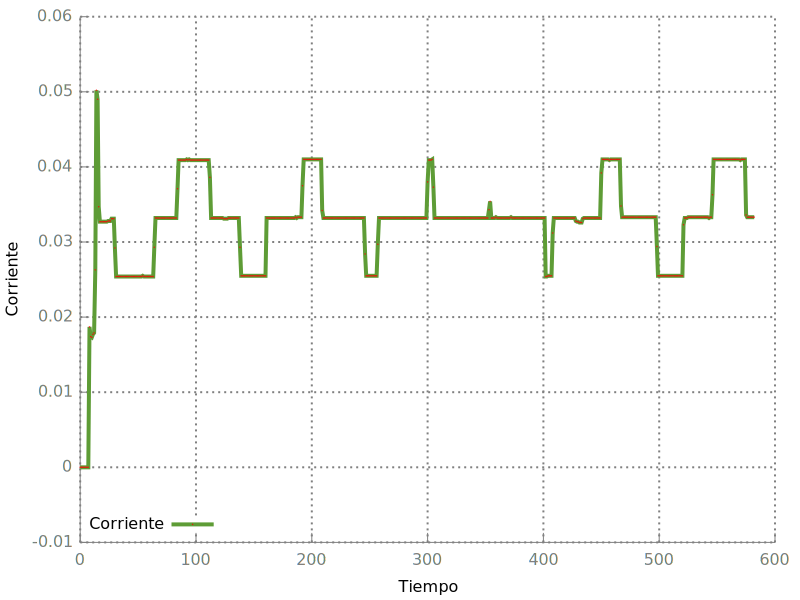
\includegraphics[scale=0.5]{capitulo_4_imgs/corriente_sd_connodo.pdf}
	\caption{Consumo de corriente como nodo coordinador con nodo final conectado.}
	\label{fig:coordinador_connodo}
\end{figure}

\begin{figure}
	\centering
	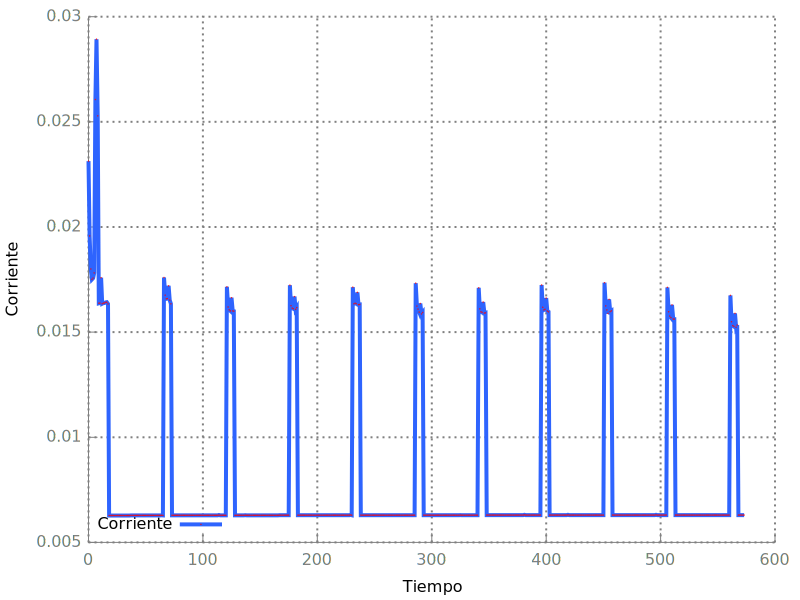
\includegraphics[scale=0.5]{capitulo_4_imgs/corriente_sd_enddevice.pdf}
	\caption{Consumo de corriente del dispositivo como nodo final.}
	\label{fig:consumo_enddevice}
\end{figure}

%Adicionalmente se realiz\'o el mismo experimento con los nodos Atmel RZRaven, detallados en el cap\'itulo 2, con el fin de comparar el consumo de corriente del dispositivo fabricado con este producto comercial. Estos resultados se pueden ver en las figuras. 

% TODO: Agregar figuras de consumo de corriente los nodos Raven.

\subsection{Medici\'on de alcance de radio comunicaci\'on}

Explicar el experimento. 
Mostrar grafica de calidad de la senial dependiendo de la distancia. 
Verificar si esta informacion esta dentro del cartel. 


\section{Pruebas de software}

Explicar distintos escenarios de pruebas del software. 
- Comunicacion con otro nodo. 
- Red de tres nodos conectados.

Execucion basica de comandos 
Ejecucion manual de comando mediante una aplicacion de trasnferencia de datos serial
- Sacar capturas de pantalla de gtkterm u otra aplicacion interactuando con el simulador. 
- 

\subsection{Aplicaci\'on de ejemplo}

- Explicar el funcionamiento basico de la aplicacion. 
-- Programa en C que: 
---- Se conecta con el dispositivo, verifica su funcionamiento.
---- Lista todos los dispositivos en la red. 
---- Envia un comando a todos los dispositivos
---- Envia un comando a una lista de nodos
---- Recibe datos de todos los nodos en la red y los imprime en pantalla. 

sd\_control --status 
sd\_control --list
sd\_control --command="1" --nodes="1234,ef43"
sd\_control --command="2" --broadcast
sd\_control --read
Ctrl+C to exit..

\subsection{Resultados de ejecuci\'on}

Capturas de pantalla del programa, mostrar algo de codigo de las secciones interesantes. 